\documentclass{beamer}

\setbeamertemplate{navigation symbols}{} % don't use navigation tools on slides

% use our .sty file for simple movie commands
\usepackage{pdfpc-commands}


\begin{document}

% Full frame movie exmaple
\frame{
    \frametitle{Example}

    Open with: \texttt{pdfpc video-example.pdf}

    \vspace{25pt}

    A full frame video using \textbf{commands from \texttt{pdfpc-commands}} is on the next slide.
}

\fullFrameMovie[loop]{apollo17.avi}{apollo17.jpg}{\copyrightText{Apollo 17, NASA}}

% Inline movie example
\frame{
    \frametitle{Example 2}

    A video using the \textbf{commands from \texttt{pdfpc-commands}} is on this slide.  The video is set to start at 5 seconds and end at 12 seconds.

    \vspace{20pt}

    \inlineMovie[loop&autostart&start=5&stop=12]{apollo17.avi}{apollo17.jpg}{height=0.7\textheight}
}

% Inline movie example
\frame{
    \frametitle{Example 3}

    A video using the \textbf{basic syntax} is on this slide.  The video is set to start at 5 seconds and end at 12 seconds.

    \vspace{20pt}

    \href{run:apollo17.avi?autostart&loop&start=5&stop=12}{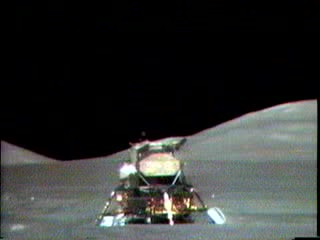
\includegraphics[height=0.7\textheight]{apollo17.jpg}}
}

\frame{
    \frametitle{Image example}

    An example full frame \textbf{image} is on the next slide.

}

% Full frame iamge example
\fullFrameImage{a17_moon.jpg}{\copyrightText{Apollo 17, NASA}}




\end{document}


